%%%%%%%%%%%%%%%%%%%%%%%%%%%%%%%%%%%%%%%%%%%%%%%%%%%%%%%%%%%%%%%%%%%%%
%% This is a (brief) model paper using the achemso class
%% The document class accepts keyval options, which should include
%% the target journal and optionally the manuscript type.
%%%%%%%%%%%%%%%%%%%%%%%%%%%%%%%%%%%%%%%%%%%%%%%%%%%%%%%%%%%%%%%%%%%%%
\documentclass[journal=jcisd8,manuscript=article,layout=onecolumn]{achemso}

%%%%%%%%%%%%%%%%%%%%%%%%%%%%%%%%%%%%%%%%%%%%%%%%%%%%%%%%%%%%%%%%%%%%%
%% Place any additional packages needed here.  Only include packages
%% which are essential, to avoid problems later. Do NOT use any
%% packages which require e-TeX (for example etoolbox): the e-TeX
%% extensions are not currently available on the ACS conversion
%% servers.
%%%%%%%%%%%%%%%%%%%%%%%%%%%%%%%%%%%%%%%%%%%%%%%%%%%%%%%%%%%%%%%%%%%%%
\usepackage[version=3]{mhchem} % Formula subscripts using \ce{}
\usepackage[numbers,sort&compress]{natbib}
\usepackage[font=scriptsize, labelfont=bf]{caption}
\usepackage{lineno}
\usepackage{rotating}
\usepackage{tablefootnote}
\usepackage{threeparttable}
\usepackage{booktabs}

%\linenumbers

%%%%%%%%%%%%%%%%%%%%%%%%%%%%%%%%%%%%%%%%%%%%%%%%%%%%%%%%%%%%%%%%%%%%%
%% If issues arise when submitting your manuscript, you may want to
%% un-comment the next line.  This provides information on the
%% version of every file you have used.
%%%%%%%%%%%%%%%%%%%%%%%%%%%%%%%%%%%%%%%%%%%%%%%%%%%%%%%%%%%%%%%%%%%%%
%%\listfiles
%%%%%%%%%%%%%%%%%%%%%%%%%%%%%%%%%%%%%%%%%%%%%%%%%%%%%%%%%%%%%%%%%%%%%
%% Place any additional macros here.  Please use \newcommand* where
%% possible, and avoid layout-changing macros (which are not used
%% when typesetting).
%%%%%%%%%%%%%%%%%%%%%%%%%%%%%%%%%%%%%%%%%%%%%%%%%%%%%%%%%%%%%%%%%%%%%

%%%%%%%%%%%%%%%%%%%%%%%%%%%%%%%%%%%%%%%%%%%%%%%%%%%%%%%%%%%%%%%%%%%%%
%% Meta-data block
%% ---------------
%% Each author should be given as a separate \author command.
%%
%% Corresponding authors should have an e-mail given after the author
%% name as an \email command. Phone and fax numbers can be given
%% using \phone and \fax, respectively; this information is optional.
%%
%% The affiliation of authors is given after the authors; each
%% \affiliation command applies to all preceding authors not already
%% assigned an affiliation.
%%
%% The affiliation takes an option argument for the short name.  This
%% will typically be something like "University of Somewhere".
%%
%% The \altaffiliation macro should be used for new address, etc.
%% On the other hand, \alsoaffiliation is used on a per author basis
%% when authors are associated with multiple institutions.
%%%%%%%%%%%%%%%%%%%%%%%%%%%%%%%%%%%%%%%%%%%%%%%%%%%%%%%%%%%%%%%%%%%%%
\author{William Fuh}
\author{Aaron T. Frank}
\email{afrankz@umich.edu}
\phone{(734) 615-2053}
\affiliation{Departments of Biophysics and Chemistry, University of Michigan, 930 North University Avenue, Ann Arbor, Michigan 48109, USA}

%%%%%%%%%%%%%%%%%%%%%%%%%%%%%%%%%%%%%%%%%%%%%%%%%%%%%%%%%%%%%%%%%%%%%
%% The document title should be given as usual. Some journals require
%% a running title from the author: this should be supplied as an
%% optional argument to \title.
%%%%%%%%%%%%%%%%%%%%%%%%%%%%%%%%%%%%%%%%%%%%%%%%%%%%%%%%%%%%%%%%%%%%%
\title[Title]
 {Identifying ``native-like'' RNA Structures Using Unassigned Chemical Shift Data}

%%%%%%%%%%%%%%%%%%%%%%%%%%%%%%%%%%%%%%%%%%%%%%%%%%%%%%%%%%%%%%%%%%%%%
%% Some journals require a list of abbreviations or keywords to be
%% supplied. These should be set up here, and will be printed after
%% the title and author information, if needed.
%%%%%%%%%%%%%%%%%%%%%%%%%%%%%%%%%%%%%%%%%%%%%%%%%%%%%%%%%%%%%%%%%%%%%
\abbreviations{NMR, RNA}
\keywords{Linear Assignment, Hungarian algorithm, RNA structure prediction, NMR spectroscopy}

\begin{document}
\begin{abstract}
In this work, we demonstrate that $\textit{unassigned}$ NMR chemical shifts, that is, an  ``anonymized'' list of observed chemical shift peak values, can be used to identify ``native-like'' conformations of RNAs.  We achieve this by casting the problem of ``assigning''  unassigned chemical shift peaks to specific sites in an RNA as a linear assignment problem, and then solve it using the fast Kuhn--Munkres  bipartite matching algorithm -- also commonly referred as the Hungarian algorithm. Using our assignment method, which we refer to as SCAHA (\underline{S}tructure-Based \underline{C}hemical-Shift \underline{A}ssignment via the \underline{H}ungarian \underline{A}lgorithm), we found that given an accurate structural model of an RNA, and chemical shift data free of referencing errors, unassigned chemical shift peaks can be assigned with an accuracy of about $\sim$0.2 and $\sim$1.0 ppm for $^{1}$H and  $^{1}$C nuclei, respectively.  By comparing SCAHA-assigned chemical shifts to computed chemical shifts, we demonstrate that we are able to identify, with high sensitivity,  ``native-like''re information to be extracted from unassigned NMR dat``native-like'' and decoy non-native structures. Our results suggest that hybrid methods that combine state-of-the-art structure prediction methods with accurate chemical shift prediction methods will soon enable RNA structure to be rapidly elucidated from \textit{unassigned} NMR spectra.
\end{abstract}
 
%%%%%%%%%%%%%%%%%%%%%%%%%%%%%%%%%%%%%%%%%%%%%%%%%%%%%%%%%%%%%%%%%%%%%
%% Start the main part of the manuscript here.
%%%%%%%%%%%%%%%%%%%%%%%%%%%%%%%%%%%%%%%%%%%%%%%%%%%%%%%%%%%%%%%%%%%%%
\section{Introduction}
The renewed appreciation of the essential and diverse roles played by ribonucleic acids (RNAs) in the cell\cite{encode2012integrated}, has led to keen interest in determining their atomistic structure. Such information is crucial to uncovering structure-function relationships that govern the regulatory properties of RNAs, and is important in the design and discovery of therapeutics that target RNAs associated with human diseases\cite{cooper2009rna}. 

$\textit{De-novo}$ structure prediction algorithms can, in principle, be used to elucidate the structure of RNAs directly from their sequence. In practice, though, additional experimental data is often needed to guide prediction efforts in what is now referred to as hybrid or integrative modeling\cite{burke2012structure, lee2016integrative}. NMR chemical shifts have recently emerge as a viable source of structural information that can be used to guide prediction of RNA structure within this hybrid modeling framework. Along these lines, Das and coworkers recently demonstrated that assigned non-exchangeable $^{1}$H chemical shift  data can, in several cases, be used to predict the structure of non-canonical motifs of RNA with near atomic accuracy\cite{sripakdeevong2014structure}. However, acquiring assigned chemical shift data, especially for medium-sized to large RNAs can be both time consuming and expensive. As such, there is keen interest in developing methods that can extract multi-resolution structural information for an RNA target directly from "unassigned" chemical shift data.

% Summarize work on utilizing unassigned data for proteins
For proteins, several methods have been developed that utilize unassigned NMR data to extract structural information. Meiler and Baker developed a method in which unassigned chemical shifts, intensities of NOESY cross-peaks, and residual dipolar couplings were used to guide protein fold prediction \cite{meiler2003rapid}. In related work, Bermejo and Llin{\'a}s described a method, referred to as SC-CLOUDS, that allowed the global fold of proteins to be determined using only unassigned NOE data. SC-CLOUDS uses a graph-theoretical approach to ``assign'' distance restraints from unassigned $^{13}$C- and $^{15}$N-edited NOESY spectra\cite{bermejo2008deuterated}. Most recently, Rienstra and coworkers developed the Comparative Objective Measurement of Protein Architectures by Scoring Shifts (COMPASS) approach in which $^{13}$C-$^{13}$C correlation spectra are simulated from structural models and then compared to a single actual unassigned  $^{13}$C-$^{13}$C correlation spectra\cite{courtney2015experimental}. In so doing, structural models can be identified that exhibit the best agreement between simulated and actual NMR spectra. For each of these methods, the folds in structural models that exhibited the best agreement with unassigned NMR data were typically in excellent agreement with the folds in known structures, and in several cases, near atomic accuracy was achieved \cite{meiler2003rapid, courtney2015experimental}. 

% Summarize work on utilizing unassigned data for RNAs
In contrast, for RNAs, few methods have been developed that enable structural information to be extracted from unassigned NMR data. One notable exception is the NMR-assisted prediction of secondary structure algorithm, referred to as NAPSS, that was  developed by Turner and coworkers. NAPSS enables secondary structure information to be extracted from unassigned NMR data\cite{hart2008nmr}. More recently, a chemical shift-based version of NAPSS, NAPSS-CS, was developed that utilizes directional chemical shift constraints to guide secondary structure prediction, and most excitingly, enabled pseudoknot RNAs to be accurately identified\cite{chen2015nuclear}. 

Currently lacking, however, are methods that enable unassigned NMR data to be incorporated into the atomistic modeling of RNAs. As has been done for proteins, state-of-the-art structure prediction algorithms could first be used to generate putative 3D models of an RNA from its sequence, and then for each generated model, unassigned chemical shift peaks could be optimally assigned to specific sites in the RNA by minimizing the difference between the chemical shifts assigned for a given site and the chemical shift computed for that site. The structural model or set of models that exhibit the best agreement between ``assigned'' and computed chemical shifts could then be identified as the predicted structure(s) of the RNA\cite{meiler2003rapid, bermejo2008deuterated, courtney2015experimental}. The success of this approach clearly hinges on the assumption that using current chemical shift prediction methods, we are able to assign chemical shifts with sufficient accuracy that enables ``native-like'' and non-native conformations of an RNA to be discriminated. Inherent in this assumption is another assumption, namely, that the ``native-like'' conformations of RNA exhibit lower assignment errors than non-native conformations of the same RNA. In this study, we set out to test the hypotheses that (1) “``native-like''” conformations of an RNA exhibit the lowest assignment errors and (2)  “``native-like''” conformations of an RNA exhibit the lowest errors between the optimally ``assigned" chemical shifts and computed chemical shifts, the latter being a more direct test of the feasibility of utilizing unassigned chemical shift to disambiguate structural differences between ``native-like'' and non-native structures of RNAs.

To test these hypotheses, we make use of a set of 52 RNAs for which NMR structures and assigned chemical shift data are available, and for which we constructed conformational pools containing both ``native-like'' and non-native decoys. To mimic unassigned chemical data, we ``anonymized'' the assigned chemical shift data and then for each RNA, applied a method we refer to as SCAHA,  \underline{S}tructure-Based \underline{C}hemical-Shift \underline{A}ssignment via the \underline{H}ungarian \underline{A}lgorithm, to optimally assign our synthetic ``anonymized'' unassigned chemical shift peaks to each structure in the conformational pools. Confirming our hypotheses, we found that in general,  the conformations that exhibited the lowest assignment errors tended to be ``native-like'', as were the conformations that exhibited the lowest errors between ``assigned" chemical shifts and computed chemical shifts. In what follows, we first describe the theoretical underpinnings of SCAHA, assess its inherent accuracy,  and finally describe in detail how we used SCAHA to test, and eventually, confirm our central hypotheses.

\section{Theoretical Methods}
\subsection{Assigning chemical shift peaks as an linear assignment problem}
The task of ``assigning'' a set of  $n$ unassigned chemical shift peaks, $\Delta^{\rm actual}\Rightarrow\{\delta_{i}^{\rm actual}\}$, to specific sites in an RNA, $S\Rightarrow\{s_{j}\}$, can be cast as a one-to-one assignment problem in which: (a) a given peak, $\delta_{i}^{\rm actual}$, can only be assigned to one site, $s_{j}$, and  (b) multiple peaks $\delta_{i}^{\rm actual}$ cannot be assigned to the same  $s_{j}$.  Formally, this assignment problem corresponds to the linear assignment problem, the optimal solution of which is the one that minimizes the objective function, $\chi$, which is defined as:
\begin{equation}\label{eq:cost} 
\chi = \sum_{i \in \Delta} \sum_{j \in S} C_{i,j} x_{i,j}
\end{equation}
where $C_{i,j}$ is the ``cost'' associated with assigning peak $\delta_{i}^{\rm actual}$ to site $s_{j}$ and $x_{i,j}$ is 1 if and only if  $\delta_{i}^{\rm actual}$ is assigned to  $s_{j}$ and 0 otherwise. Clearly, to enforce a one-to-one mapping, the the optimal solution to Eq. \ref{eq:cost} is subject to the constraints that 
\begin{equation}\label{eq:cons1} 
 \sum_{i \in \Delta}  x_{i,j} = 1 \text{ for } i \in \Delta
\end{equation}
and
\begin{equation}\label{eq:cons2} 
 \sum_{j \in S}  x_{i,j} = 1  \text{ for } j \in S.
\end{equation}
Many techniques have been developed for solving the linear assignment problem. Of note is the so-called Hungarian method, a bipartite matching algorithm which is able to solve the linear assignment problem in polynomial time\cite{kuhn1955hungarian, munkres1957algorithms} and takes as input the cost matrix \textbf{C}, whose elements are the $C_{ij}$ defined in Eq. \ref{eq:cost} and outputs the optimal assignment.
 
\subsection{SCAHA: \underline{S}tructure-Based \underline{C}hemical-Shift \underline{A}ssignment via the \underline{H}ungarian \underline{A}lgorithm} As has been done for proteins\cite{meiler2003rapid, hart2008nmr, courtney2015experimental}, unassigned chemical shift data could be incorporated into structural modeling of RNAs by optimally assigning chemical shift peaks based on a assumed structural model such that the differences between the chemical shift  peak  ($\delta_{i}^{\rm actual}$) assigned to a given site ($s_{j}$) and the chemical shift associated with that $s_{j}$ and computed from that structural model ($\delta_{i}^{\rm computed}$) are minimized.  Within such a structure-based assignment framework, the $C_{i,j}$  in  Eq. \ref{eq:cost}, which are used to construct the cost matrix (\textbf{C}), can be expressed as:
\begin{equation}\label{eq:cost_matrix} 
C_{i,j} =  \Big{|} \delta_{i}^{\rm computed} - \delta_{j}^{\rm actual}\Big{|}
\end{equation}
where $\delta_{i}^{\rm computed}$ is the chemical computed from the structural model of the RNA. The Hungarian algorithm can then be used to solve the assignment problem described by Eqs.  \ref{eq:cost}-\ref{eq:cost_matrix}. Here onward, we will refer to this general approach as SCAHA, \underline{S}tructure-based \underline{C}hemical-Shift \underline{A}ssignment via the \underline{H}ungarian \underline{A}lgorithm.

\section{Computational Details}
\label{sec:2}

Challenge sets that contained a mixture of ``native-like'' and non-native structural models were constructed for 52 RNAs, for which both NMR structures and chemical shifts were available in the PDB\cite{bernstein1977protein}  and either from literature or the BMRB\cite{ulrich2008biomagresbank}, respectively. Each of these RNAs contained non-canonical structural features (e.g., bulges, internal loops, apical loops, and three-way junctions). As such they seems as an excellent test case for The conformational pools were generated as follows: First, for each RNA, the primary sequence was extracted from its PDB file. Next, the 9 most energetically favorable secondary structures, as predicted using MC-fold\cite{parisien2008mc}, were used to generate base-pair restraints. These, along with base-pair identified in the first model of NMR bundle for a given RNA, were then used to generate structural model using Rosetta's FARNA structure prediction method\cite{das2010atomic}. For each FARNA run, 50 models were assembled and the number of cycles was set to 10000.  In addition, molecular dynamics simulations were carried out starting for the first model from each NMR ensemble. Approximately, 2000 MD-derived conformers were added to the composite pool. The CHARMM simulation package\cite{brooks1983charmm} was used for all MD simulations, which were carried out using the GBMV implicit solvent\cite{lee2002novel, lee2003new}. For the GBMV model, we used parameters that have been shown to produce relatively stable trajectories of nucleic acids, in particular, DNA\cite{chocholouvsova2006implicit}. The ten set of models returned by FARNA, together with individual models of the NMR bundle for a given RNA, and the MD generated structures were combined, and then between 25-30 conformers that evenly spanned the RMSD range between 0 and 7 \AA\  were selected. These 25-30 conformers were then used for the analysis described and discussed below. The set of conformers (referred to as the RNA-NMR decoy set) are made available via https://github.com/atfrank/RNA-NMR-Decoys.

For each of the 52 RNAs included in our analysis, unassigned chemical shift data was generated from assign chemical shift data. To  ``anonymized''  the list of assigned chemical shifts, information about residue numbers, residues names, and nucleus types were removed for the assigned chemical shift data files, thus resulting in a list of observed chemical shift peak values for each RNA (void of any information that would identify the sites to which they were assigned). Then for each conformer in the conformational pool, we then applied our SCHAHA methodology to reassign the chemical shifts to specific site in the RNA. This was achieved using the Hungarian algorithm implemented in the function {\texttt{solve\_LSAP}} in the R package clue\cite{hornik2005a}. The input to the function was a cost matrix containing elements $C_{ij}$ (Eqs. \ref{eq:cost} and \ref{eq:cost_matrix}), in which the $\delta_{\rm actual}$ and $\delta_{\rm computed}$ correspond to the ``anonymized''  chemical shifts and chemical shifts computed from the conformations in the conformational pool using either the chemical shift predictors RAMSEY\cite{frank2013prediction} or LARMOR$^{\rm D}$\cite{frank2014simple}, respectively. As such, SCHAHA was separately applied using either chemical shifts computed with RAMSEY\cite{frank2013prediction} or LARMOR$^{\rm D}$.

\begin{table}[h!]
\centering
\begin{threeparttable}
\begin{tabular}{c c c c | c c c c}
\hline
\hline

PDB & BMRB  & confomers & \# $\delta^{\rm actual/computed}$ &  PDB & BMRB  & confomers & \# $\delta^{\rm actual/computed}$ \\
\hline
\hline
1Z2J & 6543  & 26 & 425/689 & 1KKA & 5256  & 30 & 293/261 \\
2KOC & 5705  & 30 & 333/216 & 2N6S & 25780 & 30 & 308/566 \\
1YSV & 6485  & 30 & 409/423 & 2M24 & 18894 & 30 & 343/451 \\
1OW9 & 5852  & 30 & 436/349 & 1SCL & n/a  & 25 & 327/441 \\
1NC0 & 5655  & 30 & 360/368 & 2N4L & 25671 & 27 & 172/835 \\
2LDL & 17671 & 30 & 341/419 & 2MFD & 19545 & 30 & 339/295 \\
1LDZ & 4226  & 30 & 585/456 & 2M22 & 18892 & 30 & 369/355 \\
1LC6 & 5371  & 30 & 276/370 & 2QH4 & 7405  & 30 & 289/278 \\
1PJY & 5834  & 30 & 254/334 & 2N2P & 25604 & 20 & 353/363 \\
1UUU & n/a  & 30 & 273/295 & 2MEQ & 18975 & 30 & 288/293 \\
2LU0 & 18503 & 26 & 636/757 & 2M21 & 18891 & 30 & 341/327 \\
2LHP & 17860 & 30 & 282/573 & 2LQZ & 18336 & 30 & 287/419 \\
2LDT & 17682 & 27 & 204/473 & 2K66 & 15859 & 30 & 252/340 \\
2LPA & 18240 & 30 & 114/233 & 1XHP & 6320  & 30 & 425/494 \\
4A4U & 18035 & 30 & 88 /157 & 2QH2 & 7403  & 30 & 291/370 \\
2LV0 & 18549 & 30 & 408/372 & 2N2O & 25603 & 27 & 387/363 \\
2LP9 & 18239 & 30 & 120/248 & 2M12 & 18838 & 30 & 290/355 \\
2LBL & 17565 & 30 & 183/263 & 2JWV & 15538 & 30 & 480/453 \\
2FDT & 10018 & 30 & 178/560 & 2NCI & 26024 & 30 & 273/430 \\
4A4T & 18034 & 30 & 89 /158 & 2MXL & 25416 & 30 & 166/599 \\
2LK3 & 17972 & 30 & 247/370 & 2M5U & 19081 & 30 & 179/342 \\
2LBJ & 17563 & 30 & 198/261 & 2N6T & 25781 & 27 & 314/662 \\
1L1W & 5321  & 30 & 165/439 & 2MNC & 19887 & 30 & 100/248 \\
4A4S & 18036 & 30 & 89 /157 & 2M4W & 19024 & 29 & 257/261 \\
2LUB & 18515 & 25 & 277/571 & 2LUN & 18532 & 29 & 486/432 \\
2LI4 & 17877 & 27 & 232/494 & 1ZC5 & 6633  & 28 & 649/629 \\
\hline
\end{tabular}
\begin{tablenotes}
\item[1] Listed for each RNA in the challenge set are the PDB accession code, the BMRB number, number of diverse conformers in its conformation pool, the number of actual experimental/computed chemical shift peaks.
\item[2] For 1UUU, chemical shift data was obtained from literature\cite{sich1997structure}.
\item[3] For 1SCL, chemical shift data was obtained from literature\cite{szewczak1995sarcin}.

\end{tablenotes}
\end{threeparttable}
\caption{\label{tab:testing_set}  Challenge set RNAs used in this study.}
\end{table}

For each RNA, after assigning the ``unassigned'' chemical shift data to each conformer in the associated conformational pool using SCAHA, three sets of analyses were carried out:  First, to assess the accuracy of SCAHA, the assigned chemical shifts obtained by applying SCAHA to the conformer corresponding to the representative solution structure (taken as model 1 in the NMR bundle obtained from the PDB) for a given nucleus was compared to actual experimental assignment in the reference data obtained from the BMRB or directly from literature sources. For each RNA, the mean-absolute-error (MAE) over all the non-exchangeable $^{1}$H and $^{13}$C nucleus was then calculated and used as a measure of the assignment accuracy. Second, to determine whether ``native-like'' conformations had the lowest assignment errors, for given RNA in the challenge set, the MAE (see above) was calculated for each conformer in its conformational pool, and then the conformer with the lowest assignment error was identified and compared with the representative solution structure by computing the all-atom structural RMSD between the selected (``best'')  structure and the representative NMR structure. And third, to determine whether ``native-like'' conformations exhibited the smallest difference between SCAHA-assigned chemical shifts and computed chemical shifts, for given RNA in the challenge set, the weighted mean absolute error ($w$MAE) was calculated for each conformer in its conformational pool, and then the conformer with the smallest $w$MAE was identified and compared with the representative solution structure by computing the all-atom structural RMSD between the selected (``best'')  structure and the representative NMR structure. For comparison.  Here the $w$MAE is given by:

\begin{equation}\label{eq:wmae} 
w{\rm MAE} =  \frac{1}{N} \sum_{i=1}^{N} w_{i} \Big{|} \delta_{i}^{\rm assigned} - \delta_{i}^{\rm computed}\Big{|}
\end{equation}
where $\delta_{i}^{\rm assigned}$ and $\delta_{i}^{\rm computed}$ are the SCAHA-assigned and computed chemical shift associated with site $i$ ($s_{i}$) in the RNA, respectively; $N$ is the total number of sites corresponding to non-exchangeable $^{1}$H or $^{13}$C nuclei in the RNA for which ``unassigned'' chemical shifts were assigned to using SCAHA; and $w_{i}$ is a weight factor that is equal to 1/$\sigma_{i}$, where $\sigma_{i}$ is the expected accuracy with which chemical shifts are computed for the nucleus type associated with $s_{i}$\cite{frank2016can}. For comparison, the conformer that exhibited the small $w$MAE between experimentally assigned and computed chemical shifts was determine for each RNA and then compared to the results obtained using the SCAHA-assigned chemical shifts. \textit{This corresponds to the limiting case in which assignments are perfect.} In all cases, chemical shifts were computed for non-exchangeable $^{1}$H and $^{13}$C nuclei using the empirical chemical shifts predictors LARMOR$^{\rm D}$ and RAMSEY, and then the results obtained with each were then compared.

Because several of RNAs in our challenge set are known to contain systematic referencing errors\cite{aeschbacher2012procedure}, we developed an objective structure-based approach for identify such cases. To identify these ``referencing errors'' for a given RNA in our challenge set, chemical shifts were computed from the representative solution of that  RNA and then secondary chemical shifts, defined as the difference between computed and  observed chemical shifts was fitted to linear model using Bayesian regression approach implemented in the MCMCpack package in R\cite{martin2011mcmcpack}. For a given RNA, the linear model describing the secondary shift of a given nucleus $i$ of type $k$ is given by:
\begin{equation}\label{eq:wmae} 
\delta^{\rm secondary}_{i, k} =  \delta^{\rm computed}_{i, k} - \delta^{\rm actual}_{i, k} = \beta_{i, k}
\end{equation}
where $\delta^{\rm computed}_{i, k}$, $\delta^{\rm actual}_{i, k}$, $\delta^{\rm secondary}_{i, k}$, and $\beta_{i, k}$ are the chemical shift computed from the representative solution structure of that RNA, the actual chemical shift,  the secondary, and  is the fitting parameter (the intercept) associated wit $i^{th}$ nucleus of type $k$ in the RNA. Here $k$ is one of the non-exchangeable $^{13}$C nuclei in RNA, namely, C1', C2', C3', C4', C5', C2, C5, C6, C8 non-exchangeable nuclei. Within this scheme, systematic errors manifest themselves as large $\beta_{k} \equiv \langle\beta_{i, k} \rangle$, where $\langle\cdot \rangle$ denote an average over all instances of nucleus type $k$ in the dataset. For a given RNA in our challenge set, a $^{13}$C nucleus type is identified as having a referencing error if and only if $\beta_{k}$  $>$ 2.00 ppm  and $\beta_{k}$/$\sigma_{k}$ $>$ 5 (where $\sigma_{k}$ is the standard deviation of  $\beta_{i, k}$). For all RNAs in our challenge set, $^{13}$C ``referencing errors'' identified using this approach and then be used to correct the that original chemical shift dataset before converting the data into ``unassigned'' data. Here we report results using uncorrected (raw) unassigned chemical shift and corrected unassigned chemical shift data. Separately set of referencing errors were determined using chemical shift computed with LARMOR$^{\rm D}$ and RAMSEY and they are reported in Table \ref{tab:referrors}. The data and R code  used to identify these referencing errors are available at: https://github.com/atfrank/SCAHA.

\section{Results and discussion}
\begin{figure}[h!]
  \centering
       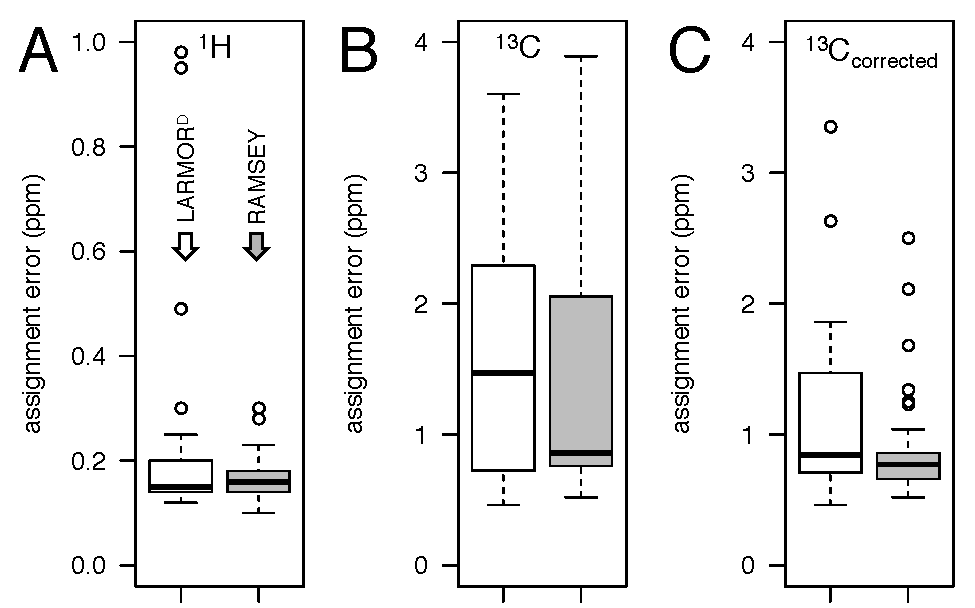
\includegraphics[width=1.0\textwidth]{figure_1}
  \caption{\textbf{Assignment Errors.} Shown are boxplots that summarize the distribution of assignment errors obtained for (A) $^{1}$H and (B and C) $^{13}$C. For $^{13}$C nuclei, results are shown when (B) SCAHA was applied using ``unassigned'' chemical shift peaks obtained directly from the BMRB and literature source and (C) SCAHA was applied using ``unassigned'' chemical shift peaks that were corrected  directly from the BMRB and literature source.}
  \label{fig:bar}
\end{figure}

We were first interested in assessing the accuracy with which a set unassigned chemical shift peaks ($\Delta^{\rm actual}\Rightarrow\{\delta_{i}^{\rm actual}\}$) could be assigned to specific sites ($S\Rightarrow\{s_{j}\}$) in each of the 52 RNAs we examined in the current study (which we refer to as our challenge set). For each RNA in our challenge set, SCAHA was applied using chemical shifts computed ($\Delta^{\rm computed}\Rightarrow\{\delta_{i}^{\rm computed}\}$) from a representative NMR structure (model 1 in the NMR bundle obtained from the PDB) using the chemical shift predictors LARMOR$^{\rm D}$ and RAMSEY  (two fast empirical chemical shift prediction methods  that are capable of predicting chemical shifts for both $^{1}$H and $^{13}$C non-exchangeable nuclei in RNA). The mean assignment errors for non-exchangeable $^{1}$H and $^{13}$C nuclei were then determined.
	
\subsubsection{For $^{1}$H nuclei, assignment errors are on-par with the inherent errors in computed $^{1}$H chemical shifts.}  Figure \ref{fig:bar}A show the distributions of mean assignment errors for $^{1}$H non-exchangeable nuclei in our challenge set. When using LARMOR$^{\rm D}$ computed chemical shifts to carry out SCAHA (LARMOR$^{\rm D}$-based SCAHA), the median assignment error was 0.15 ppm and the interquartile range was 0.06 ppm. Similar results were obtained when RAMSEY computed chemical shifts were used to carry out SCAHA (RAMSEY-based SCAHA). In this case, the median assignment error and interquartile ranges were 0.16 and 0.04 ppm, respectively. 

Because some of the RNAs included in our challenge set were also used to train LARMOR$^{\rm D}$ and RAMSEY, we were concerned that these initial estimates of the assignment errors (present above) may contain significant bias. Of the 52 RNAs contained in our challenge set, 17 of them were included in the training database used to develop LARMOR$^{\rm D}$ and 10 of them were included in the training database used to develop RAMSEY. To examine the extent to which assignment errors are affected by whether or not the RNAs in our challenge set were also used to train the predictors, we did following: for LARMOR$^{\rm D}$-based SCAHA, we analyzed separately the assignment errors for the RNAs that were in the LARMOR$^{\rm D}$ training set and those that were not included in the LARMOR$^{\rm D}$ training set. Similarly,  for RAMSEY-based SCAHA, we analyzed separately the assignment errors for the RNAs that were in the RAMSEY training set and those that were not included in the RAMSEY training set.

In Table \ref{tab:accuracy}, we compared the median assignment errors and interquartile ranges we observed for those RNAs tha were included and those that were not included in the LARMOR$^{\rm D}$ and RAMSEY training sets, respectively. For both LARMOR$^{\rm D}$ and RAMSEY, we observed marginal differences between the two sets. For example, for LARMOR$^{\rm D}$-based SCAHA,  the median assignment error and interquartile range, were 0.14 and 0.03 ppm and 0.17 and 0.08 ppm for RNAs included and not included, in the LARMOR$^{\rm D}$ training set, respectively. Similar results were about using RAMSEY (Table \ref{tab:accuracy}). On the basis of this analysis, it appears as if the estimates of the $^{1}$H assignment errors for LARMOR$^{\rm D}$- and RAMSEY-based SCAHA exhibit little unbiased with regard to  whether or not the RNAs in used in the accuracy analysis were included in the LARMOR$^{\rm D}$ and RAMSEY training database, respectively.

Interestingly, the estimated assignments errors of about $\sim$0.15 and $\sim$0.16 ppm that are associated with LARMOR$^{\rm D}$- and RAMSEY-based SCAHA, compare favorably with the expected errors of $\sim$0.15\cite{frank2014simple} and $\sim$0.14 ppm\cite{frank2013prediction} in chemical shifts computed with LARMOR$^{\rm D}$ and RAMSEY, respectively. Therefore, at least for $^{1}$H nuclei, the accuracy with which SCAHA could assign the set of unassigned chemical shift peaks  to specific sites in the RNAs in our challenge set is on-par with the estimated accuracy with which $^{1}$H chemical shifts are computed from structural models of RNAs.
\begin{table}[h!]
\centering
\caption{Assignment Accuracy}
\begin{threeparttable}
\begin{tabular}{c c c c c c c c c}
\toprule
{} &  \multicolumn{2}{c}{\textbf{$^{1}$H}} & {} & \multicolumn{2}{c}{\textbf{$^{13}$C}} & {} & \multicolumn{2}{c}{\textbf{$^{13}$C_{\rm corrected}}} \\   
dataset & $\Delta \delta$ (ppm) & IQR (ppm)  & {} & $\Delta \delta$ (ppm) & IQR (ppm) & {} & $\Delta \delta$ (ppm) & IQR (ppm)   \\
\hline
\\
all & 0.15/0.16 & 0.06/0.04 & {} & 1.47/0.86 & 1.56/1.29 & {} & 0.84/0.77 & 0.76/0.20 \\
training & 0.14/0.16 & 0.03/0.01 & {} & 0.67/0.77 & 0.16/0.66 & {} & 0.71/0.74 & 0.29/0.66 \\
not training & 0.17/0.16 & 0.08/0.06 & {} & 2.02/0.99 & 1.76/1.53 & {} & 1.13/0.78 & 0.73/0.13 \\
\\
\hline
\end{tabular}
\begin{tablenotes}
\item[1] $\Delta\delta$ and IQR is the median assignment error and interquartile range.
\item[2] Separate analyses carried out using all RNAs in challenge set (all), challenge set RNAs \textit{included} in the LARMOR$^{\rm D}$ and the RAMSEY training sets (training), and challenge set RNAs \textit{not included} in the LARMOR$^{\rm D}$ and the RAMSEY training sets (not training).
\item[3] Separated by `/' are  results associated with LARMOR$^{\rm D}$- and RAMSEY-based SCAHA assignments.

\end{tablenotes}
\end{threeparttable}
\label{tab:accuracy} 
\end{table}
\subsubsection{After Accounting for Referencing Errors, $^{13}$C Assignment Errors are also On-par with the inherent errors in computed $^{13}$C chemical shifts} For $^{13}$C nuclei, the median $^{13}$C assignment error was 1.47 and 0.86 ppm when SCAHA was carried out utilizing LARMOR$^{\rm D}$ and RAMSEY computed chemical shifts, respectively, and the interquartile range was 1.56 and 1.29 ppm, respectively. These results indicate that, RAMSEY was able to more accurately and robustly assign chemical shift peaks for  $^{13}$C nuclei. These results are not too surprising comparatively simple distance-based model the LARMOR$^{\rm D}$ uses to estimate chemical shift from structure. RAMSEY, in contrast, predicted chemical shifts using more sophisticated machine-learning based algorithm (random forest) and rich feature set that explicitly including information that includes, but not limited to, ring current effects, electrostatic bond polarization, magnetic anisotropy, hydrogen bonding and stacking. 

Compared with the expected errors in computed chemical shifts,   0.81 and 0.84 ppm, for LARMOR$^{\rm D}$ and for RAMSEY,  respectively, the assignment errors we observed, which range between $\sim$1.0 to $\sim$1.5 ppm, are larger. However, several of the $^{13}$C chemical shift datasets we used in this study are known to contain referencing errors. One would expect, therefore, that the existence of such error would significantly compromise  any of our attempts to assign these chemical shift peaks using SCAHA and result in larger than expected assignment errors.  As such, we repeated the SCAHA assignments using ``unassigned'' chemical shifts that were corrected prior to being ``annoymized'' (Table \ref{tab:referrors}).  

\begin{table}[h!]
\centering
\caption{Estimated Referencing Errors}
\begin{threeparttable}
\begin{tabular}{c c c c c c c c c c c}
\hline   
Method & PDB ID & C1' & C2' & C3' & C4' & C5' & C2 & C5 & C6 & C8  \\
\hline
LARMOR$^{\rm D}$ & 1SCL & 2.70 & 2.71 & 2.27 & 2.93 & n/a & 2.36 & 2.38 & 2.77 & 2.94 \\
LARMOR$^{\rm D}$ & 1UUU & n/a & n/a & n/a & n/a & n/a & 2.31 & n/a & n/a & n/a \\
LARMOR$^{\rm D}$ & 1XHP & 2.49 & 2.08 & 2.14 & 2.10 & 2.25 & n/a & n/a & n/a & 2.19 \\
LARMOR$^{\rm D}$ & 1ZC5 & 2.46 & 2.53 & n/a & 2.09 & 2.49 & n/a & n/a & n/a & n/a \\
LARMOR$^{\rm D}$ & 2JWV & n/a & n/a & n/a & n/a & n/a & n/a & 2.01 & n/a & n/a \\
LARMOR$^{\rm D}$ & 2K66 & 2.45 & n/a & n/a & n/a & n/a & 2.52 & 2.09 & 2.77 & 2.40 \\
LARMOR$^{\rm D}$ & 2M21 & 2.57 & 2.83 & 2.53 & 2.98 & 2.53 & 2.90 & 3.83 & 2.74 & 2.73 \\
LARMOR$^{\rm D}$ & 2M24 & 6.05 & 5.90 & n/a & n/a & n/a & 5.41 & 5.23 & 4.83 & 5.15 \\
LARMOR$^{\rm D}$ & 2M4W & 2.56 & 2.75 & 3.10 & 2.90 & 3.33 & 3.21 & 2.36 & 2.65 & 2.86 \\
LARMOR$^{\rm D}$ & 2MEQ & 2.99 & 2.58 & n/a & 2.54 & 2.95 & 3.03 & 3.04 & 3.11 & 3.10 \\
LARMOR$^{\rm D}$ & 2N6S & 2.34 & n/a & n/a & n/a & n/a & 3.72 & 3.00 & 3.01 & 3.02 \\
LARMOR$^{\rm D}$ & 2N6T & 2.40 & n/a & n/a & n/a & n/a & 3.08 & 3.22 & 3.13 & 2.99 \\
LARMOR$^{\rm D}$ & 2QH2 & 2.73 & 2.72 & n/a & 2.42 & 2.14 & n/a & 2.14 & 2.49 & 2.37 \\
LARMOR$^{\rm D}$ & 2QH4 & 2.40 & 2.90 & n/a & 2.50 & 2.04 & n/a & n/a & n/a & 2.26 \\
\\
RAMSEY  & 1PJY & n/a & n/a & n/a & n/a & n/a & 2.06 & n/a & n/a & n/a \\
RAMSEY  & 1SCL & 2.61 & 2.83 & 2.99 & 3.11 & n/a & 2.27 & 2.91 & 3.05 & 3.19 \\
RAMSEY  & 1XHP & 2.21 & 2.15 & 2.31 & 2.23 & 2.23 & 2.46 & 3.07 & 2.09 & 2.29 \\
RAMSEY  & 1ZC5 & 2.34 & 2.46 & 2.07 & n/a & 2.31 & n/a & n/a & n/a & n/a \\
RAMSEY  & 2JWV & n/a & n/a & n/a & n/a & n/a & n/a & 2.02 & n/a & n/a \\
RAMSEY  & 2K66 & 2.58 & n/a & n/a & n/a & n/a & 2.53 & 2.52 & 3.31 & 2.62 \\
RAMSEY  & 2M21 & 2.77 & 2.91 & 3.07 & 2.90 & 2.85 & 3.16 & 3.00 & 2.92 & 2.84 \\
RAMSEY  & 2M24 & 5.88 & 6.32 & n/a & n/a & n/a & 5.27 & 5.29 & 5.23 & 5.20 \\
RAMSEY  & 2M4W & 2.81 & 2.98 & 3.34 & 2.96 & 2.90 & 3.14 & 2.98 & 2.65 & 3.19 \\
RAMSEY  & 2MEQ & 2.80 & 2.78 & 2.81 & 2.73 & 3.06 & 2.41 & 2.63 & 3.32 & 3.24 \\
RAMSEY  & 2N6S & 2.52 & n/a & n/a & n/a & n/a & 3.94 & 2.72 & 3.06 & 3.13 \\
RAMSEY  & 2N6T & 2.22 & n/a & n/a & n/a & n/a & 3.33 & 2.85 & 3.04 & 3.23 \\
RAMSEY  & 2QH2 & 2.44 & 2.97 & 2.38 & 2.76 & 2.34 & 2.43 & 2.63 & 2.75 & 2.85 \\
RAMSEY  & 2QH4 & 2.51 & 3.34 & 2.02 & 2.81 & 2.56 & 2.47 & 2.21 & 3.25 & 2.91 \\

\hline
\end{tabular}
\begin{tablenotes}
\item[1] Listed are RNAs in our challenge set whose chemical shifts, obtained from either the BMRB or literature sources, are predicted contain referencing errors (Methods).
\end{tablenotes}
\end{threeparttable}
\label{tab:referrors} 
\end{table}

For LARMOR$^{\rm D}$-based SCAHA, correcting the chemical shifts significantly decreased the median assignment error from 1.47 to 0.89 and  the interquartile range was from 1.56 and 0.90 ppm, respectively. For RAMSEY, the decrease in the median assignment error was less dramatic, it decreased marginal from 0.86 to 0.83 ppm. However, the decrease in interquartile range was very pronounced; it decreased from 1.29 to 0.31 ppm. Collectively, these results indicated that after accounting for references  errors in the $^{13}$C chemical shift data, the SCAHA assignment errors (of ~0.8 to 0.9 ppm) is on-par with the estimated of the inherent errors (of ~0.8 to 0.9 ppm) in the chemical shift predictors  used in this study.  

\begin{figure}[h!]
  \centering
       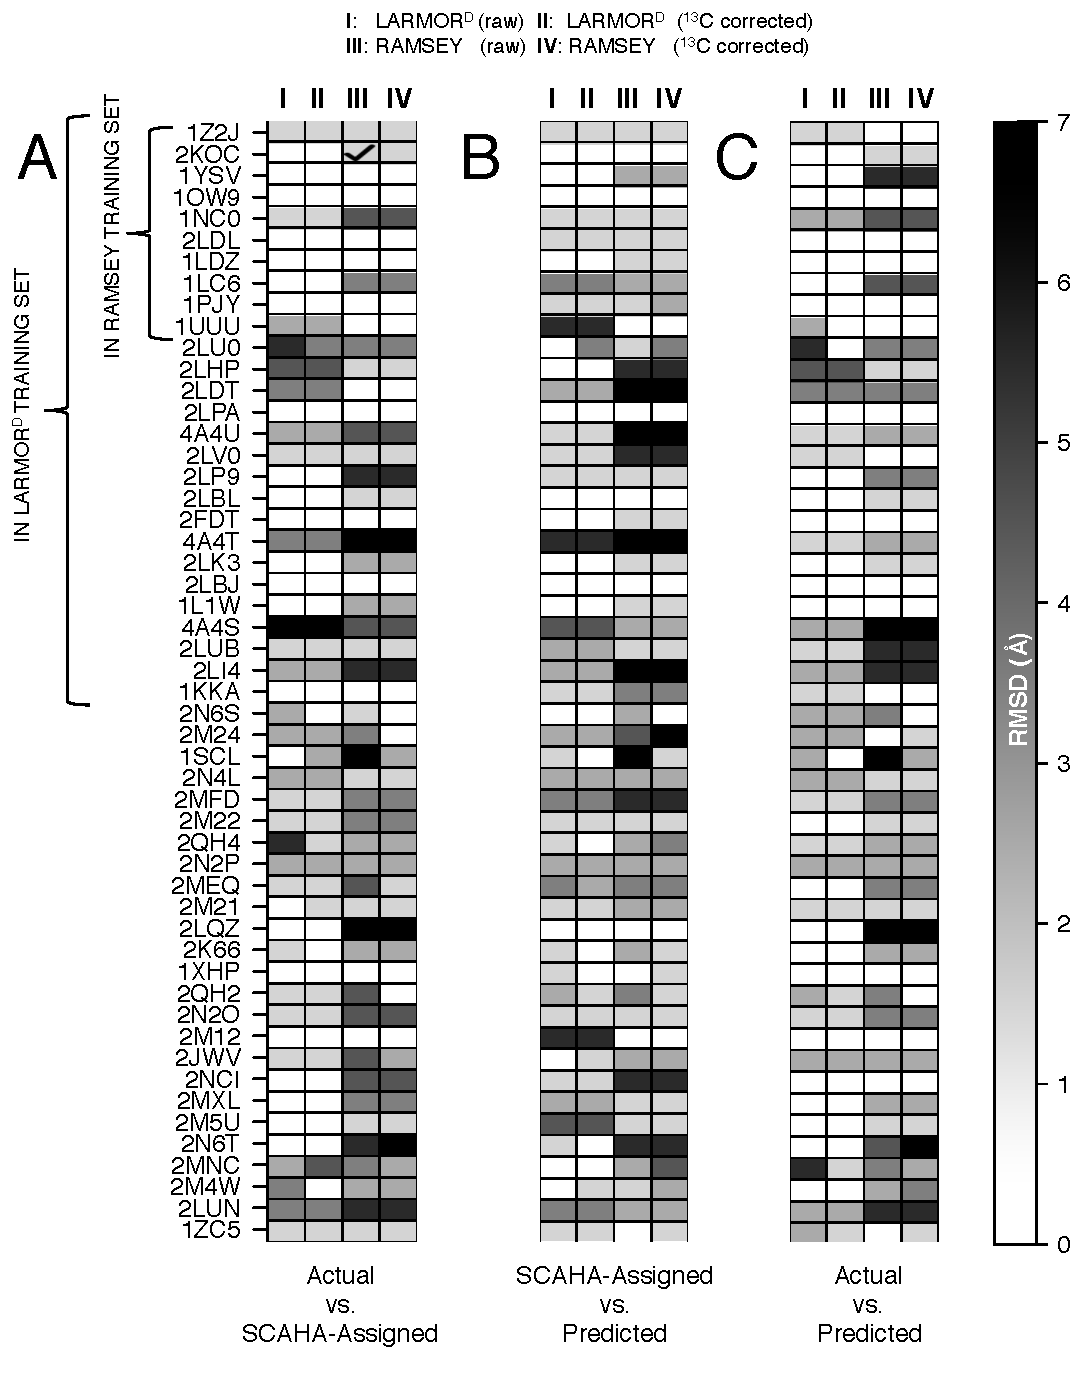
\includegraphics[width=0.8\textwidth]{figure_2}
  \caption{\textbf{Comparison between ``best'' (i.e, low-error) structures and representative solution NMR structures of RNAs in our challenge set.} Shown are levelplots of the RMSD between the representative solution NMR structure of each RNA in our challenge set and the conformer in the conformational exhibiting (A) the lowest mean absolute error (MAE) between actal experimentially assigned chemical shifts and the SCAHA-assigned chemical shifts, (B)   the lowest weighted mean absolute error ($w$MAE; Eq. \ref{eq:wmae}) between SCAHA-assigned chemical shifts and computed chemical shifts, and (C) the lowest$w$MAE between actual experimentally-assigned chemical shifts and computed chemical shifts. For each levelplot, results are shown when using LARMOR$^{\rm D}$ computed chemical shifts  and (column \textbf{I}) raw uncorrected chemical shifts data and  (column \textbf{II}) corrected chemical shifts data (Methods), and RAMSEY computed chemical shifts  and (column \textbf{III}) raw uncorrected chemical shifts data and  (column \textbf{IV}) corrected chemical shifts data, respectively. Indicated (upper left) are the RNAs in our challenge set that were included in the datasets used to train LARMOR$^{\rm D}$ and RAMSEY, respectively. Note that only $^{13}$C chemical shift re-referenced (where appropriate; see Methods)}
  \label{fig:levelplot}
\end{figure}

As we did for $^{1}$H nuclei, we also investigated the impact on our assessment of the assignment errors. In contrast to $^{1}$H, however, we did observe a significant difference in the assignment errors for those RNAs included in the training database of LARMOR$^{\rm D}$ and RAMSEY, and those that were not included. For example, for LARMOR$^{\rm D}$, even after accounting for referencing errors, the median assignment errors for RNAs included it's training database was 0.71 ppm, compared with a value of 1.13 ppm for those RNAs in our testing set that were not included in the LARMOR$^{\rm D}$ training database.  Additionally, the interquartile ranges were dramatically different, for RNA included in the training database the IQR value was only 0.29 ppm, compared to 0.90 ppm for RNAs not included in the training database. For RAMSEY, similar results were obtained.

\subsubsection{SCAHA Assignments are Rarely ``Perfect''} 
As a further gauge of the overall performance of SCAHA, for each RNA in our challenge set, we determined the fraction of the assignments that were perfect ($f_{\rm perfect}$), that is, the fraction SCAHA assignments that matched the actual experimental assignments. In general, we found that the $f_{\rm perfect}$ values were very small.  For example, for LARMOR$^{\rm D}$ and RAMSEY-based SCAHA, the median $f_{\rm perfect}$ (calculated over all the RNAs in our challenge set) were only 0.066 (6.6 \%) and 0.057 (5.7 \%), respectively  (Table \ref{tab:fractions}). Similar results were also obtained for the RNAs the were included and those not included in the LARMOR$^{\rm D}$ and RAMSEY training sets, respectively (Table \ref{tab:fractions}). Similarly, we also computed the fractions of assignments that were less than the expected prediction errors ($f_{\rm < error}$). For LARMOR$^{\rm D}$ and RAMSEY-based SCAHA, the median $f_{\rm < error}$ (calculated over all the RNAs in our challenge set) were 0.596 (59.6 \%) and 0.528 (52.8 \%), respectively  (Table \ref{tab:fractions}). For the RNAs the were included and those not included in the LARMOR$^{\rm D}$ and RAMSEY training sets, respectively, the corresponding values were 0.639 (63.9 \%) and 0.536 (53.6 \%) and 0.548 (54.8 \%) and 0.521 (52.1 \%), respectively (Table \ref{tab:fractions}). 

\begin{table}[h!]
\centering
\caption{Mean RMSD between the ``best'' (i.e, low-error) structure and the representative solution NMR structure for RNAs in our challenge set.}
\begin{threeparttable}
\begin{tabular}{*5c}
\hline
dataset & {} & $f_{\rm perfect}$ & {} & $f_{\rm < error}$ \\
\hline
all & {}           & 0.066/0.057 & {} & 0.596/0.528 \\
training & {}      & 0.078/0.075 & {} & 0.639/0.536 \\
not training & {}  & 0.059/0.057 & {} & 0.548/0.521 \\
\hline
\end{tabular}
\begin{tablenotes}
\item[1]  $f_{\rm perfect}$: median fraction of perfect assignments
\item[2] $f_{\rm < error}$: median fraction of assignments less than the associated prediction error
\item[3] Separated by `/' are  results associated with LARMOR$^{\rm D}$- and RAMSEY-based SCAHA assignments.
\end{tablenotes}
\end{threeparttable}
\label{tab:fractions} 
\end{table}

\subsubsection{Though SCAHA Assignments are Rarely ``Perfect'',  ``Native-Like'' Structures Appear to Exhibit the Lowest Assignment Errors} 


Though the fraction of perfect assignment made by SCAHA are typically small, the fact that $\sim$50 \% of the assignments were within the expected errors  in the computed chemical shifts suggest that it  might still be possible to use structure-based assigned chemical shifts to guide structural modeling of RNA. Indeed, previous work on proteins have demonstrated that even when there are assignment discrepancies between the structure-based assignments and the actual, experimental assignments\cite{meiler2003rapid, bermejo2008deuterated, courtney2015experimental}, unassigned NMR data could still be used acquire structural information about proteins by identifying structure or set of structures that exhibited the smallest difference between optimally assigned and computed chemical shifts. 

Accordingly, given the current accuracy with which SCAHA could be used to assign unassigned chemical shift, we then tested the first of the hypotheses described in the introduction, namely, that “``native-like''” conformations of an RNA exhibit the lowest assignment errors. To test this hypothesis, for each RNA in our challenge set we optimally assigned the unassigned chemical shifts using SCAHA to each of the conformations associated with that RNA. For each nucleus in a given RNA for which chemical shift data was available, we compared the SCAHA-assigned chemical shift to the actual, experimentally assigned chemical shift, computed the mean absolute assignment error for each conformation, and then identify the ``best'' conformation as the one exhibiting the lowest assignment error. If our hypothesis is correct, then we would expect that for the majority of RNAs in our challenge set, the ``best'' conformation is ``native-like''. Indeed, this is what we observed (Figure \ref{fig:levelplot}; Table \ref{tab:meanrsmd}). For LARMOR$^{\rm D}$-based SCAHA, the mean RMSD for the ``best'' conformation was 1.53 and 1.53 \AA when prior to and after correcting for $^{13}$C referencing errors, respectively. For  RAMSEY-based SCAHA, the corresponding values were 2.66 and 2.34 \AA, respectively.

Given that some of the RNAs in our challenge set were included in the training sets used to develop LARMOR$^{\rm D}$ and RAMSEY, we carried out separate analyses for RNAs in our challenge set that were included in the respective training sets and those that were not included in those training sets. For RAMSEY-based SCAHA,  when comparing the results for RNAs that were included in the RAMSEY training set and those that were not included, we observed an increase in the mean RMSD of the ``best'' conformations: using uncorrected chemical shift data, the mean RMSD of the ``best'' conformations was 1.41 and 2.96 \AA, respectively. 

Interestingly, for LARMOR$^{\rm D}$-based SCAHA,  we did not observed such a large discrepancy when comparing the results for RNAs that were included in the training the LARMOR$^{\rm D}$ and those that were not included: using uncorrected chemical shift data, the mean RMSD of the ``best'' conformations were both 1.53 and 1.53 \AA, respectively. Taken together, these results indicate that in general, and especially for LARMOR$^{\rm D}$-based SCAHA, the conformation of an RNA that exhibit the lowest assignment error do tend to be ``native-like''. Here we note that the training set used to train RAMSEY predictors only contained 19 RNAs, as compared to 36 RNAs for LARMOR$^{\rm D}$. As such, this difference probably explains why LARMOR$^{\rm D}$-based SCAHA appeared to be more robust than RAMSEY-based SCAHA performance of LARMOR$^{\rm D}$ and RAMSEY: LARMOR$^{\rm D}$ predictors were trained on a more large and diverse set of RNAs and so is more sensitive to structural differences in these RNAs. (Counterintuitively, it was RAMSEY-based SCAHA that was able to more accurately assigned the ``unassigned'' chemical shift data (Figure \ref{fig:bar}).)

\begin{figure}[h!]
  \centering
       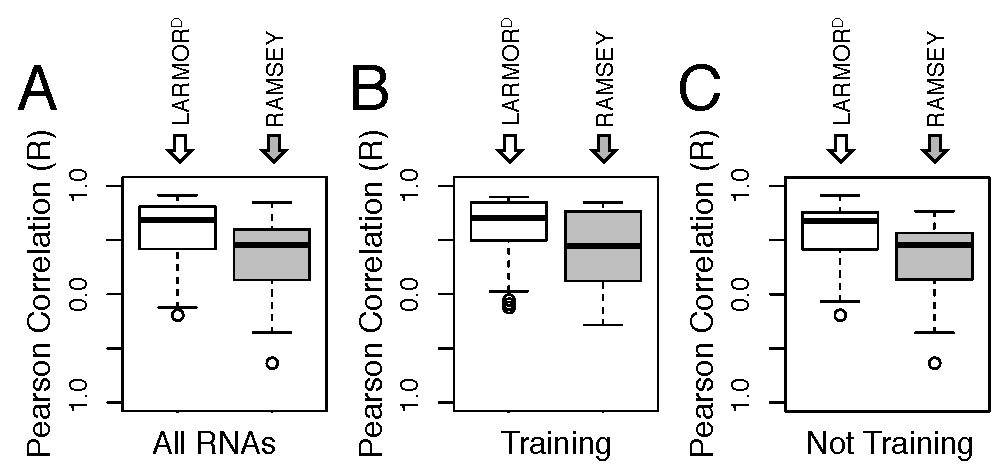
\includegraphics[width=0.8\textwidth]{figure_3}
  \caption{\textbf{Assessing the ability to identifying ``native-like'' conformations} XXX}
  \label{fig:correlations}
\end{figure}

The use of structured-based assignment approaches to first assign unassigned chemical shift peaks and then identify ``native-like'' conformations of RNA hinge on the assumption that the non-nativeness (e.g., as measured by the RMSD) is positively correlated with assignment error. In other words, it hinges on the assumption that the more non-native the conformation the larger the assignment error. To investigate more closely this relationship between assignment error and structure, for each RNA in our challenge set, we determined the extent to which assignment error was correlated to structural (dis)similarity relative to the representative solution structure. 

Shown in Figure \ref{fig:correlations} is are distributions of the Pearson correlation coefficient ($R$) between the assignment error and the structural RMSD. Overall, we observed a positive correlation between the assignment errors associated with both LARMOR$^{\rm D}$- and RAMSEY-based SCAHA exhibited a positive correlation with the ``non-nativeness'', and these results did not depend on whether or not the RNAs were included in the LARMOR$^{\rm D}$ and RAMSEY training sets: over all the RNAs in our challenge set, the median $R$ between the RMSD and LARMOR$^{\rm D}$- and RAMSEY assignment errors were 0.68  and 0.46, respectively;  over the RNAs in the included in the LARMOR$^{\rm D}$ and RAMSEY training sets, respectively, these values 0.70 and  0.44; and over the RNAs in the not included in the LARMOR$^{\rm D}$ and RAMSEY training sets, these values 0.67 and 0.46. Though both the assignment errors associated with both LARMOR$^{\rm D}$- and RAMSEY-based SCAHA exhibited a positive correlation with the ``non-nativeness'', the correlations is strongest for LARMOR$^{\rm D}$, which is consistent with our observations that the assignment errors associated LARMOR$^{\rm D}$-based SCAHA were better able to identify ``native-like'' conformations of RNAs.

Taken together, the results presented above show that though the fraction of perfect assignments that achieved with SCAHA are low, the conformations of each RNA in our challenge set that exhibit the lowest assignment errors do indeed tend to be native-like.

\subsubsection{``Native-like'' Structures Also Exhibit the Lowest Chemical Errors Between SCAHA-Assigned and Computed Chemical Shifts.} Encouraged by the fact that ``native-like'' structures exhibit the lowest assignment errors, and that there was a positive correlation between assignment error and ``non-nativeness'', we next addressed the second hypothesis laid out in the introduction, namely, that “``native-like''” conformations of an RNA exhibit the small differences (errors) between ``assigned" and computed chemical shifts. Within a structured-based assignment framework, in which unassigned data is assign to specific sites in an RNA by assuming a structural model of an RNA and then optimally assigning the unassigned data based on chemical shifts computed from that structure, the more direct test of the feasibility of utilizing unassigned chemical shift to identify native like structures is whether the conformations of an RNA that exhibit the smallest difference between the optimally ``assigned'' and computed chemical shifts are ``native-like''. If, in general, the conformation(s) that exhibits the small difference between ``assigned'' and computed chemical shifts are indeed ``native-like'', then it would suggest that unassigned chemical shift data could be used to together with RNA structure prediction approaches to identify ``native-like'' conformations, thus enabling useful structural information about an RNA to be acquired from unassigned chemical shift data.
\begin{table}[h!]
\centering
\caption{Mean RMSD between the ``best'' (i.e, low-error) structure and the representative solution NMR structure for RNAs in our challenge set.}
\begin{threeparttable}
\begin{tabular}{*9c}
\toprule
{} & \multicolumn{2}{c}{\underline{Actual vs. Assigned}} & {} & \multicolumn{2}{c}{\underline{Assigned vs. Predicted}} & {} & \multicolumn{2}{c}{\underline{Actual vs. Predicted}} \\
dataset & LARMOR$^{\rm D}$   & RAMSEY   & {} & LARMOR$^{\rm D}$  & RAMSEY   & {} & LARMOR$^{\rm D}$    & RAMSEY \\

\hline
all & 1.53/1.43 & 2.66/2.34 & {} & 1.73/1.67 & 2.54/2.60 & {} &  1.38/1.07 & 2.35/2.22 \\
training & 1.53/1.47 & 1.41/1.41 & {} & 1.38/1.53 & 1.47/1.52 & {} &  1.30/1.09 & 1.69/1.69 \\
not training & 1.53/1.40 & 2.96/2.57 & {} & 2.06/1.79 & 2.80/2.86 & {} &  1.46/1.06 & 2.51/2.35 \\
\hline
\end{tabular}
\begin{tablenotes}
\item[1] RMSD are reported in \AA.
\item[2] Separated by `/' are  results associated with raw uncorrected chemical shift data and corrected chemical shift. Note that only $^{13}$C chemical shift re-referenced (where appropriate; see Methods); $^{1}$H chemical shift used as reported in the BMRB or literature sources.  
\end{tablenotes}
\end{threeparttable}
\label{tab:meanrsmd} 
\end{table}

We therefore repeated  the analysis described above, but instead of calculating the differences between SCAHA-assigned chemical shifts and the experimentally assigned chemical shifts, we calculated the differences between SCAHA-assigned chemical shifts and LARMOR$^{\rm D}$ and RAMSEY computed chemical shifts. The results we obtained mirrored closely the results that was obtained when comparing SCAHA-assigned chemical shifts to experimentally assigned chemical shifts. For example, over the entire set of RNAs in our challenge set, for LARMOR$^{\rm D}$- and RAMSEY-based SCAHA, the mean RMSD of the ``best'' conformations (i.e., those that exhibit the smallest differences) were 1.73 and  and 2.54 \AA, respectively when using the uncorrected $^{13}$C data and 1.67 and 2.60 \AA\, respectively when using corrected $^{13}$C data. %By comparison, when comparing SCAHA-assigned chemical shifts and the experimentally assigned chemical shifts, these values were 1.53 and  and 2.66 \AA, respectively and 1.43 and  and 2.34 \AA, respectively. 
For RNAs included in the LARMOR$^{\rm D}$ and RAMSEY training, these values were 1.38 and  and 1.47 \AA, respectively when using the uncorrected chemical shift data and 1.53 and 1.52 \AA\, respectively when using the corrected chemical shift data. For RNAs not included in the training sets, the corresponding values were 2.06 and  and 2.80 \AA, respectively and 1.79 and 2.86 \AA\, respectively. 

Comparing computed chemical shifts to the actual, experimental assigned chemical shifts, enabled us to assess the ability to identify ``native-like'' in the limit of ``perfect'' assignment (or when fully assigned chemical shift is available). For RNAs not included training sets, the mean RMSD of the ``best'' conformations based on LARMOR$^{\rm D}$- and RAMSEY-based SCAHA were 1.46 and  and 2.51 \AA, respectively when using the uncorrected chemical data, and 1.06 and 2.35 \AA, respectively when using the corrected chemical data, compared with the values of 2.06 and  and 2.80 \AA, respectively and 1.79 and 2.86 \AA\, respectively that obtained using SCAHA-based assignments. 

Focusing on the results obtained for RNAs not included in the training sets and utilizing data free of referencing, the results we obtain indicate that: (i) Starting from completely unassigned chemical shift data, SCAHA-based assignments could be used to identify  ``native-like'' structures of RNA in our challenge set to within $\sim$2.0 and 3.0 \AA\ when using LARMOR$^{\rm D}$ and RAMSEY computed chemical shifts, respectively;  and (ii) In the limit of perfect assignment (or when fully assigned chemical shift data is available) ``native-like''  structures could be identified to within $\sim$1.0 and 2.5 \AA\ when using LARMOR$^{\rm D}$ and RAMSEY computed chemical shifts, respectively.

\begin{table}[h!]
\centering
\caption{Mean RMSD between five ``best'' (i.e, five low-error) structures and representative solution NMR structures of RNAs in our challenge set.}
\begin{threeparttable}
\begin{tabular}{*9c}
\toprule
{} & \multicolumn{2}{c}{\underline{Actual vs. Assigned}} & {} & \multicolumn{2}{c}{\underline{Assigned vs. Predicted}} & {} & \multicolumn{2}{c}{\underline{Actual vs. Predicted}} \\
dataset & LARMOR$^{\rm D}$   & RAMSEY   & {} & LARMOR$^{\rm D}$  & RAMSEY   & {} & LARMOR$^{\rm D}$    & RAMSEY \\

\hline
all & 1.76/1.70 & 2.77/2.56 & {} & 1.99/1.99 & 2.93/2.95 & {} & 1.51/1.52 & 2.57/2.43 \\
training & 1.59/1.57 & 2.25/2.25 & {} & 1.76/1.80 & 2.76/2.77 & {} & 1.50/1.50 & 1.93/1.93 \\
not training & 1.92/1.82 & 2.89/2.64 & {} & 2.19/2.17 & 2.97/2.99 & {} & 1.52/1.53 & 2.73/2.55 \\
\hline
\end{tabular}
\begin{tablenotes}
\item[1] RMSD are reported in \AA.
\item[2] Separated by `/' are  results associated with raw uncorrected chemical shift data and corrected chemical shift. Note that only $^{13}$C chemical shift re-referenced (where appropriate; see Methods); $^{1}$H chemical shift used as reported in the BMRB or literature sources.  
\end{tablenotes}
\end{threeparttable}
\label{tab:meanrsmd} 
\end{table}

Collectively, the results we presented above suggest that unassigned chemical shift data may find utility in guiding structural modeling of RNAs within a framework in which structure prediction methods are first used to sample or generate putative conformations of an RNA, then a structure-based assignment method is used to optimally assign the unassigned chemical shift data to each conformation, and finally the conformation(s) that exhibit the best agreement between the optimally ``assigned'' chemical shifts and computed chemical shifts is/are identified. Similar to how assigned chemical shift data as been used to guide modeling\cite{sripakdeevong2014structure}, within this framework, the unassigned chemical shift data is used to disambiguate  structural differences between the ``native-like'' vs non-native conformations of RNAs. The results presented thus far seem to suggest that the errors between optimally ``assigned'' chemical shifts and computed chemical shifts can -- for the majority of RNAs in our challenge set -- accurately resolve these structural differences. To more directly probe this, we computed the normalized sum of logarithmic ranks (NSLR)\cite{venkatraman2010comprehensive}, a popular performance metric which quantities the ability of some ``measure''  (here, the error between SCAHA-assigned chemical shifts and computed chemical shifts) to separate or resolve groups within a dataset (here the ``native-like'' and non-native conformers in the conformational pools of the RNAs). The NSLR ranges between 0 and 1, with 1 corresponding to complete separation (or, perfect ``resolvability'') of the two groups and is well suited for quantifying the resolving power of unassigned chemical shift data over the RNAs in our challenge set\cite{frank2016can}. Figure \ref{fig:sensitivities} summarizes the results of this analysis.

In contrast to the theoretical NSLR that one would expect if the conformers in each conformational pool was randomly prior to its calculation (NSLR $\sim$ 0.50), we found that the NSLR obtained using the errors between computed chemical shifts and the chemical shifts assigned using LARMOR$^{\rm D}$ were large. For example, over the entire set of RNAs in our challenge set, the median NSLR associated with LARMOR$^{\rm D}$-based SCAHA assignments were 0.8. Similar results were obtained regardless of whether or not the RNAs that were analyzed were included the respective LARMOR$^{\rm D}$ (Figure \ref{fig:sensitivities}B and \ref{fig:sensitivities}C).  These results indicating that for most of the RNAs, the errors between the computed chemical shifts and  chemical shifts optimally assigned using LARMOR$^{\rm D}$-based SCAHA were effective at resolving structural differences between the native and non-native conformation of the RNAs in our challenge set.  In contrast, the median NSLR associated with RAMSEY-based SCAHA was consistently near $\sim$0.5 (Figure  \ref{fig:sensitivities}A, \ref{fig:sensitivities}B and \ref{fig:sensitivities}C), indicating that only about half the RNAs median NSLR in excess of what one would expect for NSLR associated random sorting of the conformation. Similarly, the NSLR obtained using the conformational energies obtained using the Rosetta all-atom energy function\cite{alford2017rosetta} tended to be $\sim$0.5; for example, over the entire challenge set the Rosetta NSLR was 0.52 for Rosetta.

Interestingly, if experimentally assigned chemical shifts are used instead of the SCAHA assigned chemical shifts and compared with computed chemical shifts, the NSLR we observed were relatively large (Figure  \ref{fig:sensitivities}D-F), indicative of strong resolving power. For example, for the RNAs not included in the LARMOR$^{\rm D}$ and RAMSEY training sets respectively, the median NSLR values were 0.90 and 0.70, respectively (Figure  \ref{fig:sensitivities}F). This is to be compared with values of 0.75 and 0.50 that are obtained using chemical shifts assigned with LARMOR$^{\rm D}$- and RAMSEY-based SCAHA, respectively (Figure  \ref{fig:sensitivities}C). Though not the central focus of this study, these results do serve to highlight potential of assigned NMR chemical shifts data in disambiguating ``native-like'' from non-native structures. In addition do serves as an indication of the limiting resolving power one might expect as more accurate structured-assignment strategies are developed.


In summary, by comparing computed chemical shifts to SCAHA-assigned chemical shifts, and then identifying the structure that exhibits the lowest difference between them, the native-like conformation could be identified for most of the RNA in our challenge set. Moreover, as evidence by larger NSLR, LARMOR$^{\rm D}$ associated chemical shifts errors exhibited a superior ability to separate (or resolve) the set of all native-like conformations with the decoy pool of each RNA from the set of non-native decoys than RAMSEY-associated errors (Figure \ref{fig:sensitivities}). More importantly, LARMOR$^{\rm D}$ chemical shifts errors also exhibited superior ability to separate (or resolve) native-like conformations from non-native decoys than the Rosetta RNA all-atom energy function (Figure \ref{fig:sensitivities}), a clear demonstration of the potential value that can be added by incorporating unassigned chemical shifts into the structural modeling of RNAs through the use of structured-based assignment approaches like SCAHA.

\begin{figure}[h!]
  \centering
       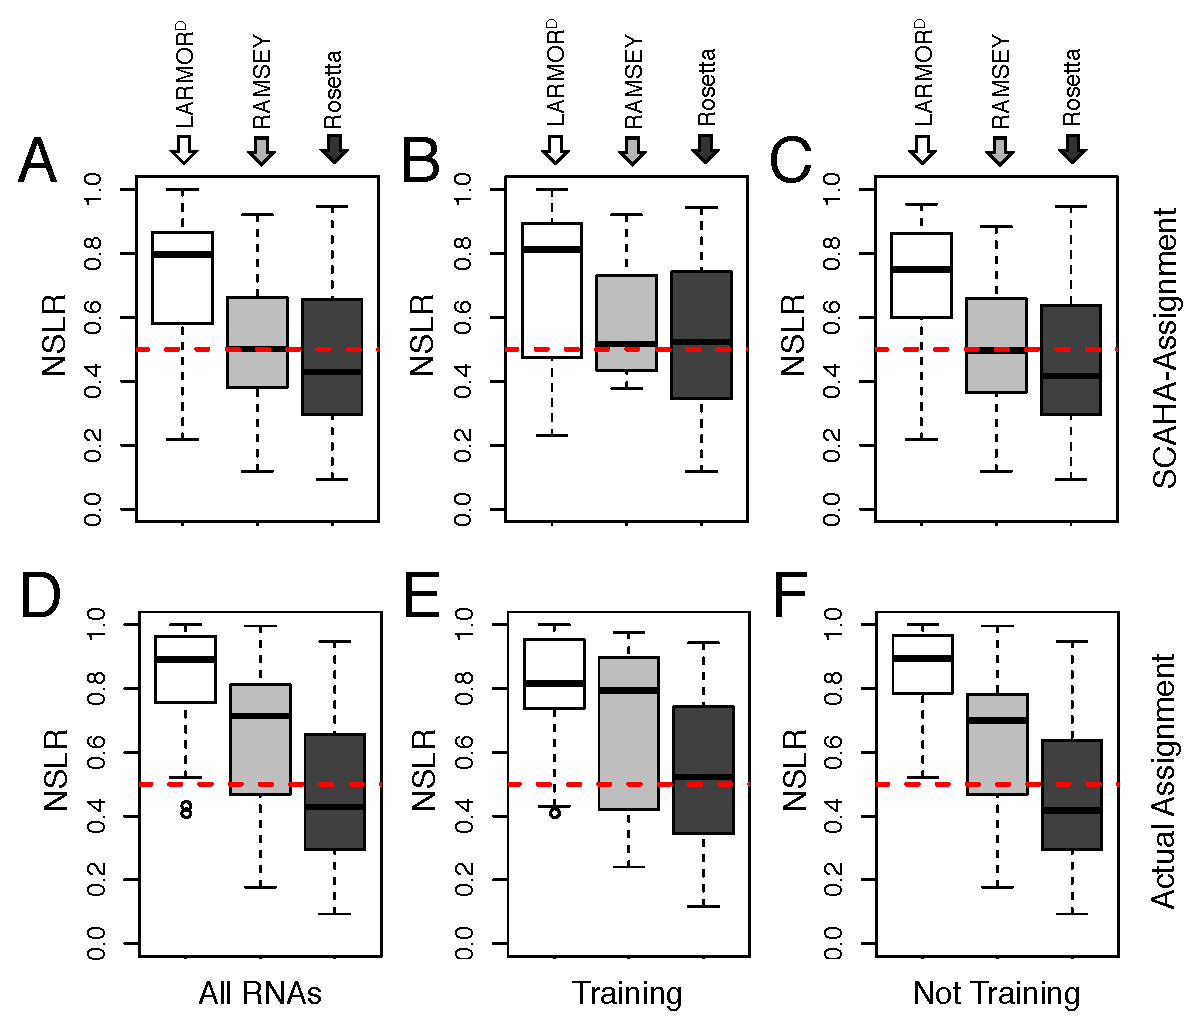
\includegraphics[width=0.9\textwidth]{figure_4}
  \caption{\textbf{Resolving ``native-like'' from non-native using unassigned chemical shift data.} Distributions of the normalized-sum-of-logarithmic ranks (NSLR) for (A, D) all the RNAs in our challenge set, (B, E) RNAs in our challenge set that were \textit{included} in the LARMOR$^{\rm D}$ and RAMSEY training set, and (C, F) RNAs in our challenge set that were \textit{not included} in the LARMOR$^{\rm D}$ and RAMSEY training set. Shown in each boxplot are the NSLRs that were obtained based on the weighted mean-absolute-error ($w$MAE; Eq. \ref{eq:wmae}) between (A-C) computed chemical shifts and chemical shifts assigned using LARMOR$^{\rm D}$- and RAMSEY-based SCAHA, respectively and (D-F) computed chemical shifts and actual experimentally assigned chemical shifts.  Also reported are the NSLR distribution obtained by using the energies obtained by minimizing and scoring conformations using the Rosetta all-atom energy function\cite{alford2017rosetta}. For reference, the NSLR that one would expect to observe if conformer are randomly sorted is indicated by the red dashed line.}
  \label{fig:sensitivities}
\end{figure}

\section{Discussion} 
Motivated by our interest in utilizing unassigned chemical shift data to aid in the structural modeling of RNAs, in the current study we focused on addressing two related hypotheses, namely, that (1) ````native-like''” conformations of an RNA exhibit the lowest assignment errors and (2)  ````native-like''” conformations of an RNA exhibit the small differences errors between optimally ``assigned" chemical shifts and computed chemical shifts. Our results, which confirm both of these hypotheses, are encouraging and bode well for the potential use of unassigned chemical shift data in modeling the 3D structure of RNAs. Similar to what has been done for proteins\cite{meiler2003rapid, bermejo2008deuterated, courtney2015experimental}, unassigned NMR data could be used to guide the modeling of RNAs by combining state-of-the-art structure prediction methods with SCAHA in a hybrid scheme in which a diverse set of RNA structures are sampled using these structure prediction methods and then SCAHA, taking as input unassigned chemical shift data, is used to identify the model(s) that exhibit the smallest difference between the optimally assigned chemical shifts and the computed chemical shifts. The results above suggest that, in general, these models tend to be ``native-like''. %However, the assignment accuracy, and the ability to identify ``native-like'' structures in our challenge set is sensitive to the presence of reference errors in the ``unassigned'' data. Such errors, however, can be mitigated by adopting the internal referencing strategy described by Aeschbacher et. al\cite{aeschbacher2012procedure}. 

Currently, the available empirical structure-based chemical shift method can confidently predict chemical shifts for non-exchangeable $^{1}$H and $^{13}$C nuclei. LARMOR$^{\rm D}$ can also, predict chemical shift imino and amino nuclei, but the prediction errors are relatively large ($\sim$0.40 and $\sim$1.32 ppm, respectively)\cite{frank2014simple} when compared to the expected errors in non-exchangeable $^{1}$H and $^{13}$C predictions ($\sim$0.15 and $\sim$0.81 ppm, respectively)\cite{frank2014simple}. As such, using empirical predictors, SCAHA can only confidently be used to assign chemical shifts for non-exchangeable $^{1}$H and $^{13}$C nuclei, even though, in a practical setting, unassigned peaks list will contain chemical shifts peaks for other $^{1}$H, $^{13}$C,  and $^{15}$N nuclei as well, depending the type of NMR experiment carried out. As an alternative, chemical shifts for all NMR-active nuclei in RNAs can be computed using quantum mechanics. However, even for small RNAs ($<$40-nt), such calculations can be computationally demanding, though recently described fragmentation schemes go a long way towards making these calculation more feasible\cite{swails2015afnmr}. The expense of these quantum mechanically calculation notwithstanding, SCAHA can be used in conjunction with quantum mechanically computed chemical shifts, thus enabling, in principle, all the observed  $^{1}$H, $^{13}$C,  and $^{15}$N peaks to be assigned.

We note that though our development of SCAHA was motivated by our interest in utilizing unassigned chemical shift data to guide modeling of RNA structure SCAHA is completely general and so can be used to assign chemical shift peaks using chemical shifts computed from structural models of \textit{any molecule}; SCAHA takes as input a simple text file containing a list of observed chemical shift peak value (which are to be assigned to specific sites in a given molecule) and a file containing chemical shifts computed from a structural model or set of models of that molecule. Beyond RNA, SCAHA can therefore also be used to assign chemical shift peaks in other biomolecules, for example, proteins, and so can be used to guiding structural modeling of those molecules.

In the current study, we did not attempt to optimize SCAHA, instead, in the current version of SCAHA we made use the Hungarian algorithm already implemented in the clue package in R\cite{hornik2005a}. In our hands, the mean SCAHA-runtime (for a single conformer) over our challenge set of 52 RNAs was 1.361 s, and the SCAHA-runtimes ranged between $\sim$0.133 to $\sim$25.96 s for RNAs that had cost matrices that contained 88 $\times$ 157  and 172 $\times$ 835 elements, respectively. In the context of modeling large RNAs, for which the use of unassigned data might be most useful, and for which the cost matrices that are inputted into the Hungarian algorithm are larger, the longer runtimes will possibly limit the number of conformations that can post-processed using SCAHA. Fortunately, a graphical processing unit (GPU)-accelerated implementation of the Hungarian algorithm was recently developed\cite{date2016gpu} and so future work will center on implementing a fast GPU-accelerated version of SCAHA. To facilitate use and further testing of the current version of SCAHA, we have released the source code under a GNU license and make it freely available to the academic community https://github.com/atfrank/SCAHA. 

\section{Conclusion}
Recent studies have demonstrated that potential of utilizing assigned chemical shift data to guide the modeling of the three-dimensional (3D) structure of ribonucleic acids (RNAs). In this study, we attempted to assess the feasibility of utilizing \textit{unassigned} chemical shift data to guide the 3D model of RNAs. As a first step toward utilizing unassigned chemical shift data to model the 3D of RNAs, we developed a structure-based assignment method, which we refer to as SCAHA, that takes as input a list of unassigned chemical shift peaks and chemical shifts computed from a structural model of an RNA and outputs the optimally assigned chemical shifts. Then, using SCAHA, we tested two hypotheses crucial to assessing the feasibility of utilizing unassigned chemical shift data in structural modeling of RNA. In particular, we tested the hypotheses that (1) ````native-like''” conformations of an RNA exhibit the lowest errors between the optimally assigned chemical shifts and actual experimentally assigned chemical shifts and (2) that ````native-like''” conformations of an RNA exhibit the small differences errors between the optimally chemical shifts and computed chemical shifts. Confirmation of these hypotheses will suggest that using unassigned chemical shift data, ``native-like'' conformers within a set containing both of ``native-like'' non-native conformers, could be identified. 

By applying SCAHA to a challenge set containing 52 RNAs, for each of which, conformational pools containing both ``native-like'' and non-native decoys were constructed, we were able to directly test these two hypotheses. We found that the conformers in the conformational pools  that exhibited the lowest assignment error tended to be ``native-like'' and likewise, the conformer that exhibited the small difference between optimally assigned chemical shifts and computed chemical tended to be ``native-like''. Taken together, these results suggest that provide that a reliably structured-based assignment model is available, then ``native-like'' conformations of RNAs could be identified from a set of putative structural models by assigning chemical shift to each of the models and then selecting the model or set of models with the lowest error between the ``assigned'' and chemical shifts computed from the models. These results should pave the way for developing workflows that combine structured-based assignment methods, like SCAHA, with modern structure prediction methods, like FARFAR, MC-Sym, RNAComposer (to name a few), in order to utilize unassigned chemical shift data guide the modeling of RNAs.

%\section{Acknowledgement}

%%%%%%%%%%%%%%%%%%%%%%%%%%%%%%%%%%%%%%%%%%%%%%%%%%%%%%%%%%%%%%%%%%%%%
%% The same is true for Supporting Information, which should use the
%% suppinfo environment.
%%%%%%%%%%%%%%%%%%%%%%%%%%%%%%%%%%%%%%%%%%%%%%%%%%%%%%%%%%%%%%%%%%%%%
%%%%%%%%%%%%%%%%%%%%%%%%%%%%%%%%%%%%%%%%%%%%%%%%%%%%%%%%%%%%%%%%%%%%%
%% The appropriate \bibliography command should be placed here.
%% Notice that the class file automatically sets \bibliographystyle
%% and also names the section correctly.
%%%%%%%%%%%%%%%%%%%%%%%%%%%%%%%%%%%%%%%%%%%%%%%%%%%%%%%%%%%%%%%%%%%%%
\bibliography{papers_library_abbreviate.bib}
%%%%%%%%%%%%%%%%%%%%%%%%%%%%%%%%%%%%%%%%%%%%%%%%%%%%%%%%%%%%%%%%%%%%%
%% The "tocentry" environment can be used to create an entry for the
%% graphical table of contents.
%%%%%%%%%%%%%%%%%%%%%%%%%%%%%%%%%%%%%%%%%%%%%%%%%%%%%%%%%%%%%%%%%%%%%

\begin{tocentry}
\centering
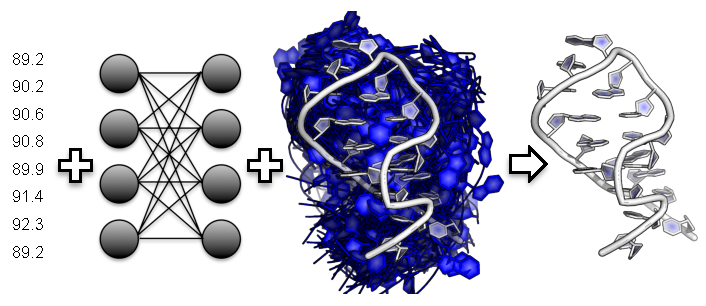
\includegraphics[width=3.3in]{toc}
Illustrating the use of unassigned chemical shift  to identify ``native-like'' structures of an RNA
\end{tocentry}

\end{document}
